 
\section{Model-fitting}

% -----------------------------------------------------------------------------
\subsection{Maximum Likelihood and Estimation Theory}
An estimator $\hat{P}(X)$ is a \textcolor{red}{function} that maps from its sample space $X$ (data) to a set of \emph{sample estimates} $W$\\
An estimator ...
   \vspace{-0.1cm}
    \begin{itemize}
    \item is a function of a random variable
    \item is a random variable 
    \item can be statistically characterized via its moments
    (mean, variance, ...)\\ $\leadsto$ quality criteria: unbiasedness, efficiency
    \end{itemize}
set of observations: $\big\{ \vec{x}^{(\alpha)} \big\}, \alpha = 1, \ldots, p$
\\\\
true distribution (normalized): 
\begin{equation}
        P\big(\big\{\vec{x}^{(\alpha)}\big\};
                \underbrace{ \vec{w}^* }_{ \substack{ 
                        \text{true} \\ 
                        \text{parameter} \\ 
                        \text{value}}} \big) \equiv P 
\end{equation}
\begin{itemize}
        \itl true model is member of the model class
        \itl structure of the postulated model has to be valid
\end{itemize}
model selection $\Rightarrow$ estimation of the ''true'' values $\vec{w}^*$ from the observed data
\\\\
estimator $\widehat{\vec{w}}$:
\begin{equation}
        \widehat{\vec{w}} = \widehat{\vec{w}}
                \big(\big\{\vec{x}^{(\alpha)}\big\}\big)
\end{equation}
\begin{itemize}
        \itl procedure for the determination of $\vec{w}^*$ given the observed
                data
        \itl $\vec{w}^*$ is a function of $\big(\big\{ 
                \vec{x}^{(\alpha)}\big\}\big)$
        \itl $\vec{x}^{(\alpha)}$ are random variables $\rightarrow 
                \widehat{\vec{w}}$ is a random variable
\end{itemize}

\paragraph{The Maximum Likelihood estimator}\mbox{}\\
\textbf{the likelihood function}\\
\begin{equation*}
        \widehat{P}\big(\big\{\vec{x}^{(\alpha)}\big\}; \vec{w}\big)
\end{equation*}
\textbf{the $\log$-likelihood function}
$$
\ln \widehat{P}\big(\big\{\vec{x}^{(\alpha)}\big\};\vec{w}\big)
= \sum\limits_{\alpha = 1}^p \ln \widehat{P}
                        \big( \vec{x}^{(\alpha)};\vec{w} \big) 
$$
\textbf{the Maximum Likelihood estimator}\\
\begin{equation*}
        \widehat{\vec{w}} = \underset{\vec{w}}{\operatorname{argmax}}\widehat{P}\big(\big\{\vec{x}^{(\alpha)}\big\}; \vec{w}\big) 
\end{equation*}

\paragraph{quality criteria for estimators:} (see also MI I, section 1.4.5)
\begin{equation}
        \begin{array}{ll}
                \text{bias:} & \vec{b} = \underbrace{ \big< 
                        \widehat{\vec{w}} \big>_p }_{
                        \substack{      \text{expectation} \\
                                        \text{w.r.t \underline{true}} \\
                                        \text{distribution}}
                                }- \vec{w}^* \\\\
                \text{variance:} & \vec{\Sigma} = \big< ( \widehat{\vec{w}}
                        -\vec{w}^*)(\widehat{\vec{w}} - \vec{w}^* )^T \big>_p
        \end{array}
\end{equation}
optimal estimators:
\begin{equation}
        \begin{array}{lcl}
                \text{no bias:} & \vec{b} \eqexcl 0 & \leftarrow
                        \substack{      \text{only possible if true model} \\
                                        \text{within model class} } \\\\
                \text{minimal variance:} & |\vec{\Sigma}| \eqexcl \min
                        & \leftarrow \substack{\text{smallest average 
                            deviation} \\ \text{of } \widehat{\vec{w}} \text{ from }
                                                \vec{w}^*}
        \end{array}
\end{equation}

\paragraph{Example}\mbox{}\\
\textbf{sample mean}\\
$N$ observations 
$
x^{(\alpha)} = A + \epsilon^{(\alpha)}
$
with $ \epsilon^{(\alpha)}\sim N(0,\sigma^2)$ \\

\textbf{Examples for estimators for A:}
\begin{align*}
\hat{A} &= \frac{1}{N} \sum x^{(\alpha)} && \text{unbiased} \\
\tilde{A} &= \frac{1}{2N} \sum x^{(\alpha)} && \text{biased for} A\neq 0 \\
\tilde{A} &= k && \text{minimum variance but biased}
\end{align*}

 

\paragraph{The minimum variance unbiased estimator}\mbox{}\\
\textbf{Optimal estimators:}
$$
	\begin{array}{lcl}
		\text{no bias:} & \vec{b} \eqexcl 0 & \leftarrow
			\substack{	\text{only possible if true model} \\
					\text{within model class} } \\\\
		\text{minimal variance:} & |\vec{\Sigma}| \eqexcl \min
			
	\end{array}
$$
MVU: criteria have to hold for ALL possible values of $\vec{w}^*$!
\vspace{5mm} 

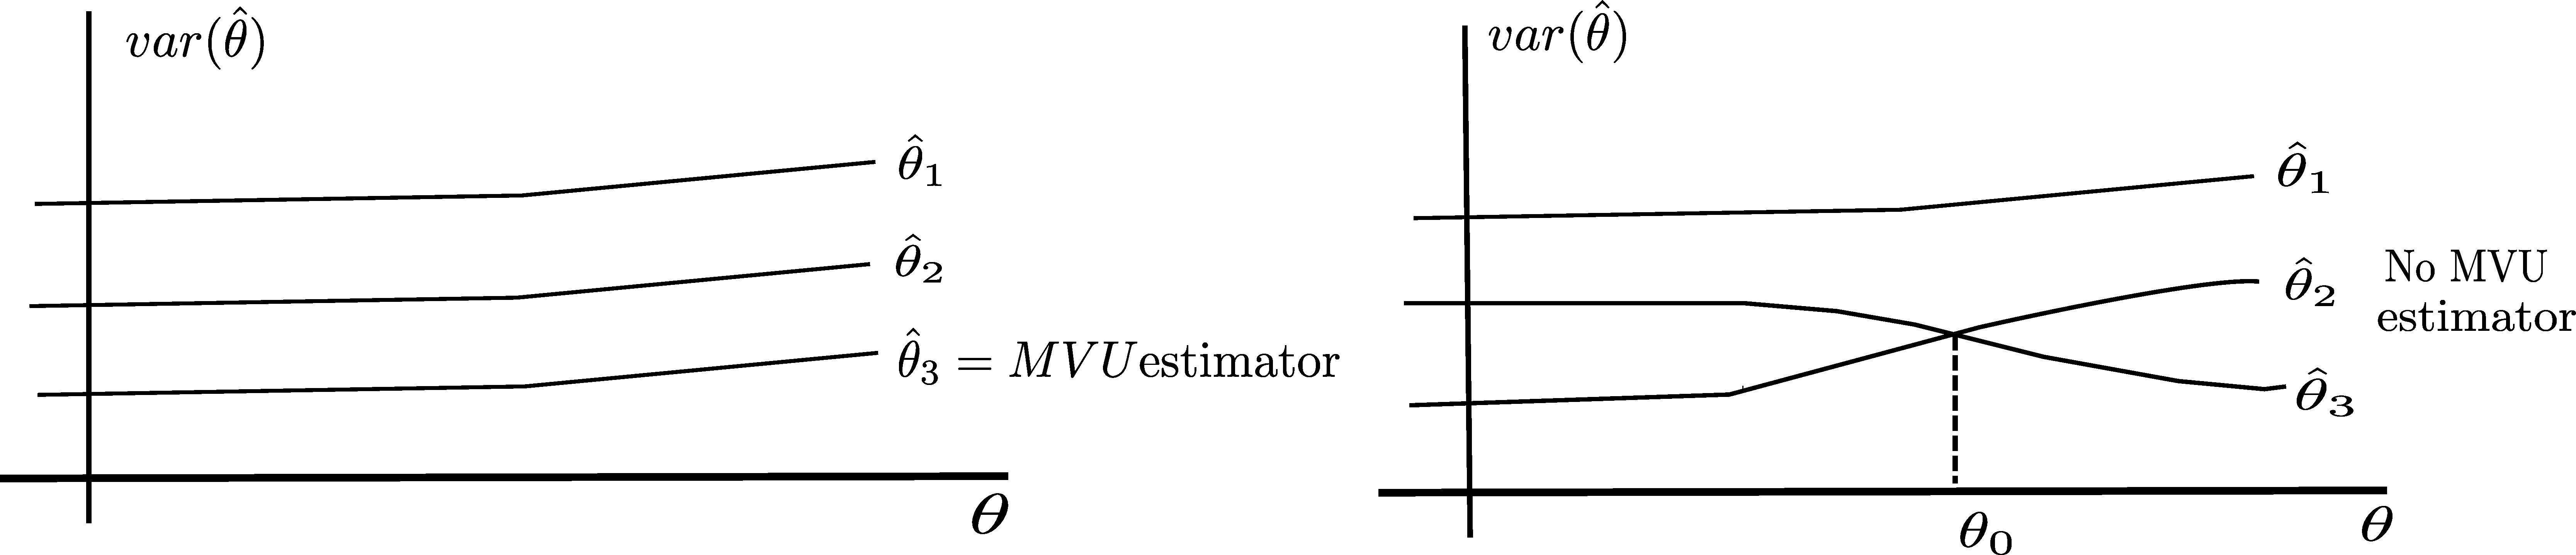
\includegraphics[width=\textwidth]{section7_fig1} \\ 
MVUs do not always exist \\

given just observed sample conditionally independent observations with the 2 pdfs
$$
x[0] \sim \mathcal{N}(\theta,1) \qquad
x[1] \sim
\left\{
\begin{array}{c}
  \mathcal{N}(\theta,1) \quad \rm if \hspace{0.2cm} \theta \geq 0 \\\\
  \mathcal{N}(\theta,2) \quad \rm if \hspace{0.2cm}  \theta < 0 
\end{array} 
\right.
$$ 
two estimators
$$
\hat{\theta}_1 = \frac{1}{2}(x[0]+x[1]) \qquad \text{and} \qquad
\hat{\theta}_2 = \frac{2}{3} x[0] + \frac{1}{3} x[1]
$$
variances: 
\begin{eqnarray*}
var(\hat{\theta}_1) & = & \frac{1}{4}(var(x[0])+var(x[1])) \qquad
\left\{
\begin{array}{c}
  \frac{18}{36} \quad \rm if \hspace{0.2cm} \theta \geq 0 \\[0.7em]
  \frac{27}{36} \quad \rm if \hspace{0.2cm} \theta < 0 
\end{array} 
\right. \\\\
var(\hat{\theta}_2) & = & \frac{4}{9} var(x[0]) + \frac{1}{9} var(x[1]) \qquad
\left\{
\begin{array}{c}
  \frac{20}{36} \quad \rm if \hspace{0.2cm} \theta \geq 0 \\[0.7em]
  \frac{24}{36} \quad \rm if \hspace{0.2cm} \theta < 0 
\end{array} 
\right.
\end{eqnarray*}
\vspace{3mm}

\paragraph{Example for the non-existence of MVUs (Kay, 1993)}
\begin{center}
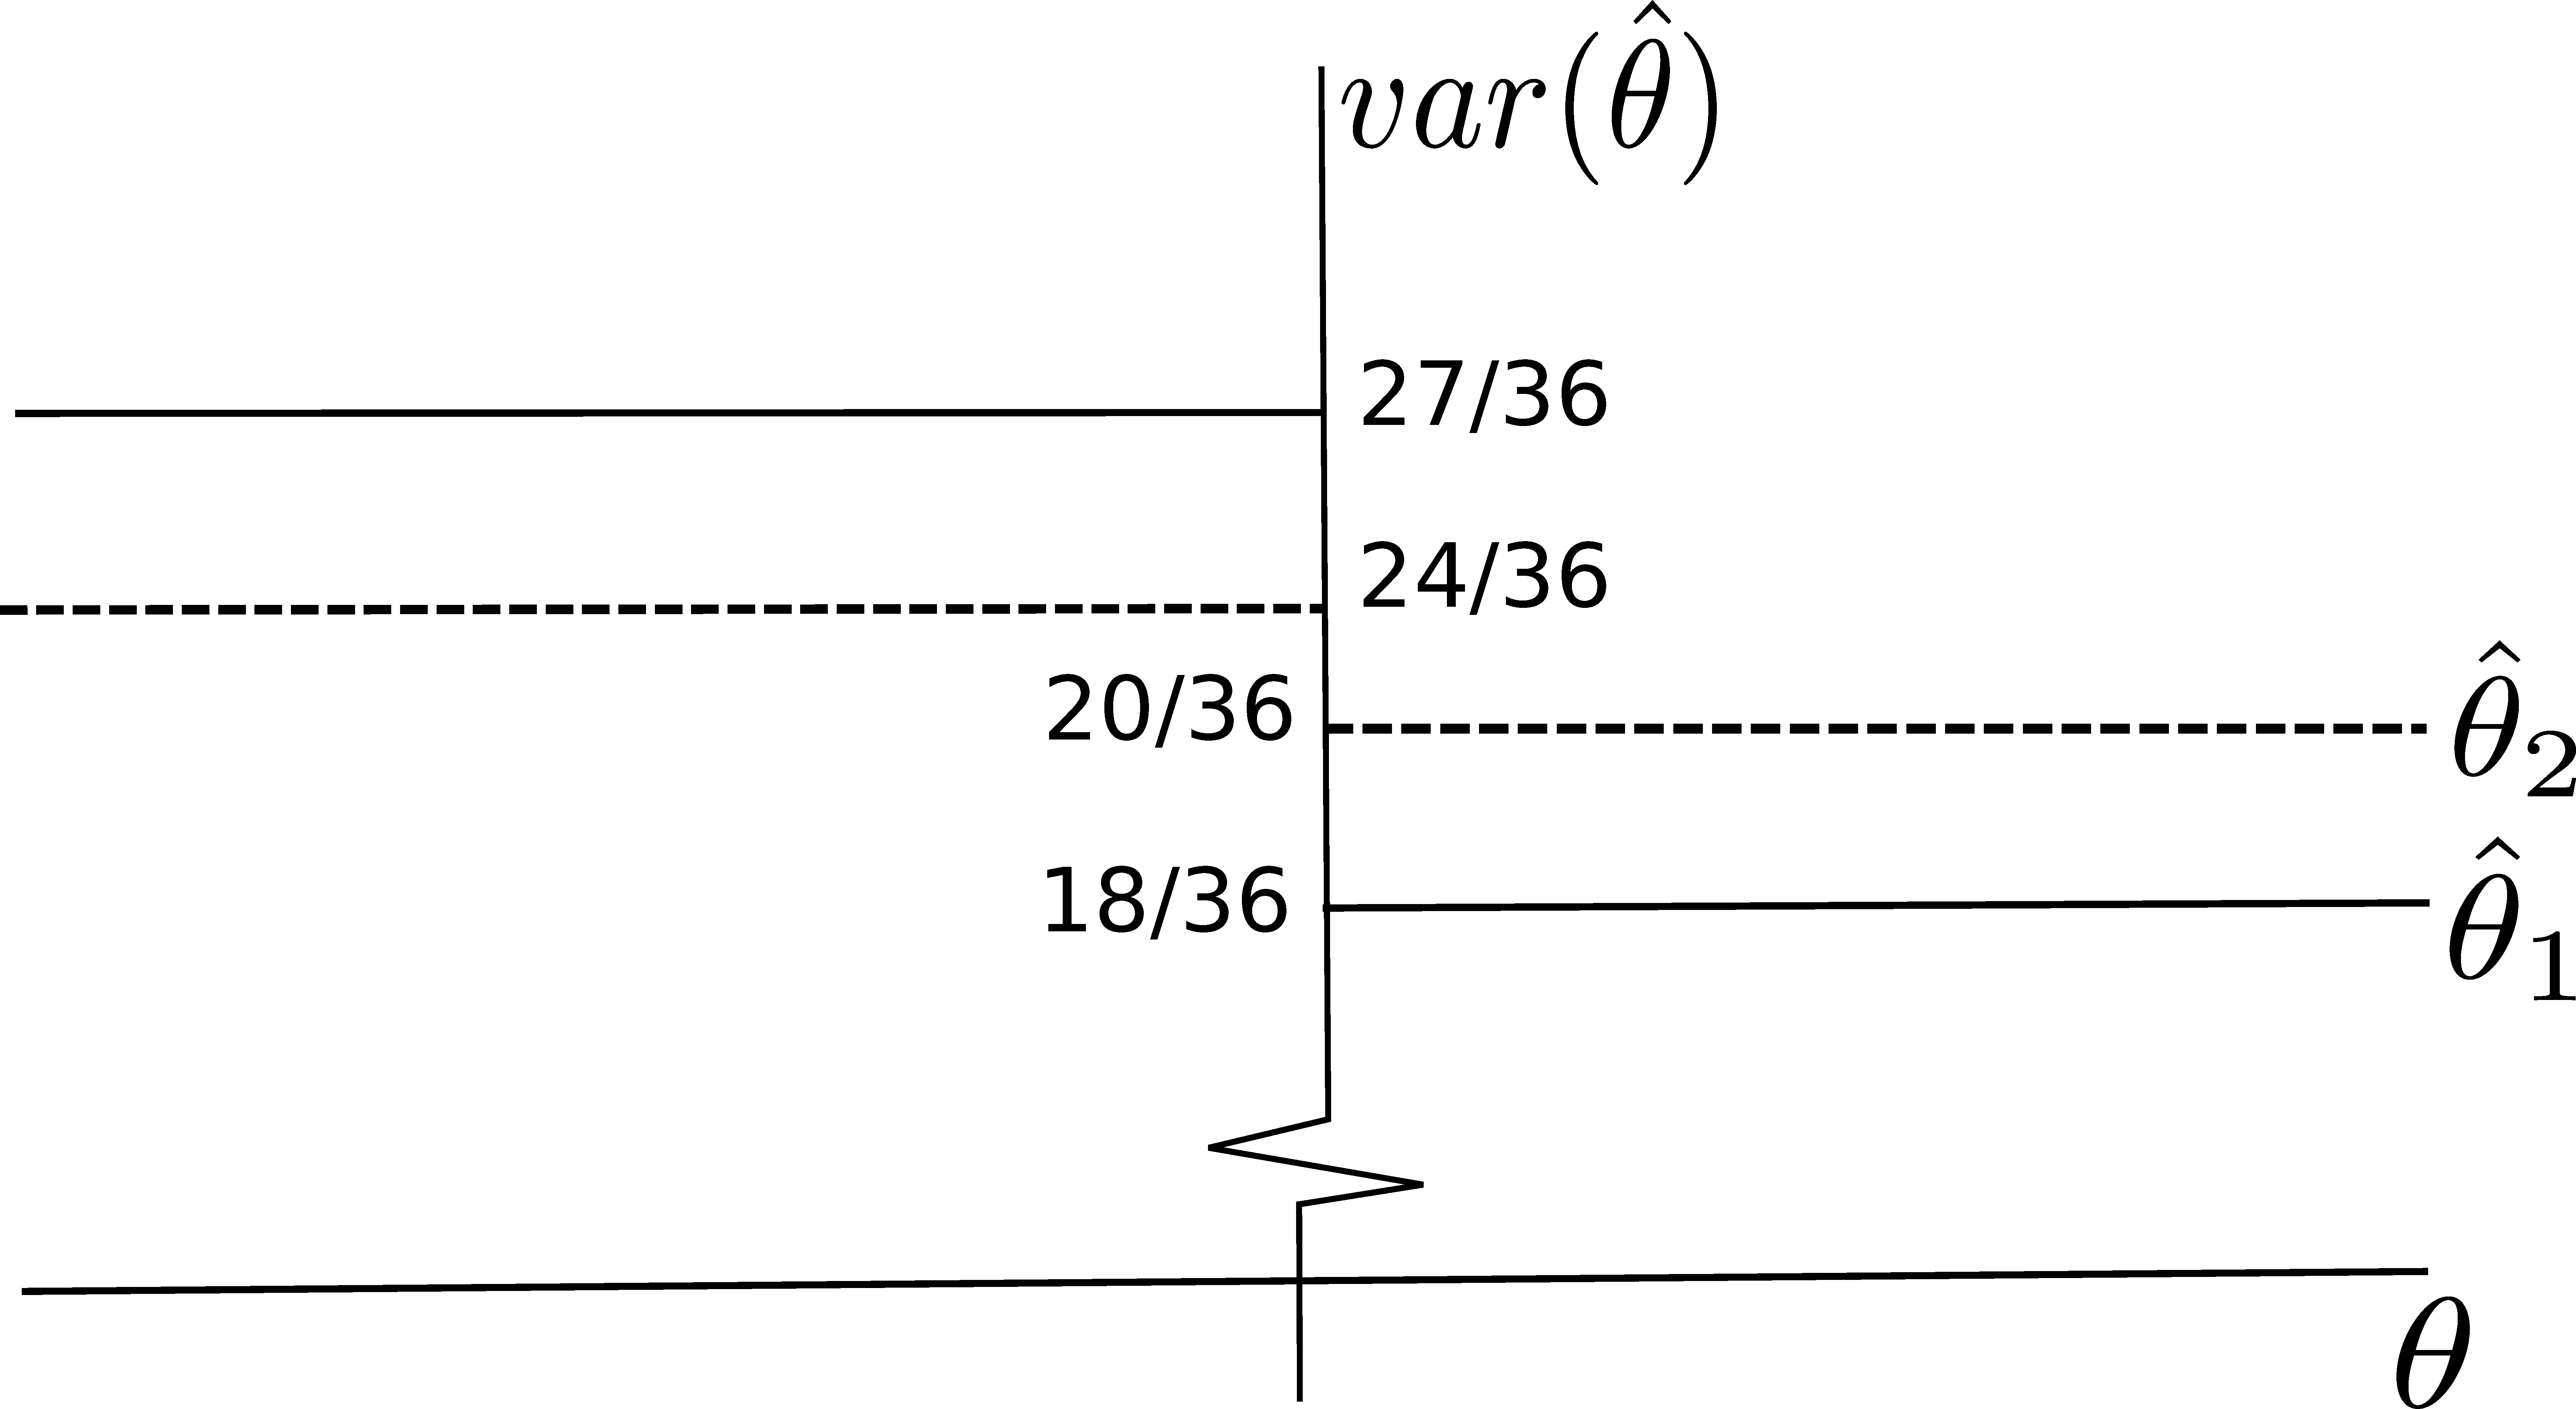
\includegraphics[width=0.75\textwidth]{section7_fig2}
\end{center}

\paragraph{MVU vs. minimal mean squared error}
$$MSE(\hat{\vec{w}}) = E[(\hat{\vec{w}}-\vec{w^*})^2]$$
\vspace{0.5cm}
This however does not yield a realizable estimator because
\begin{eqnarray*}
MSE(\hat{w}) & = & E\left\{[(\hat{w} - E(\hat{w}) ) +(E(\hat{w})-w^*) ]^2\right\}\\
 & = & var(\hat{w}) + [ E(\hat{w}) -w^* ]^2\\
 & = & variance + bias^2
\end{eqnarray*}
MSE trades bias against variance.
 
\subsection{Cramer-Rao Bound}
\paragraph{Cramer-Rao bound for unbiased estimators}\mbox{}\\
The stronger a PDF depends on its parameters, the more accurate will their estimates be.
\vspace{0.2cm}

$N$ observations $x^{(\alpha)}$ with $ \epsilon^{(\alpha)} \sim N(0,\sigma^2)$ 
$$
x^{(\alpha)} = A + \epsilon^{(\alpha)}, \hspace{1cm} \hat{A} = \frac{1}{N} \sum x^{(\alpha)} 
$$
\begin{center}
\includegraphics[width=0.8\textwidth]{section7_fig3}  
\end{center}
Accuracy can be measured by the 'sharpness' of the likelihood
  function ($\leadsto$ 2nd derivative of the neg. log likelihood).


Cramer-Rao bound for unbiased estimators:
\begin{equation} \tag{$\substack{\text{Fisher infor-}\\ \text{mation matrix} }$}
        M_{ij} = -\Bigg< \frac{\partial^2 \ln P}{\partial \mathrm{w}_i
                        \partial \mathrm{w}_j} \Bigg>_p \Bigg|_{\vec{w}^*}
\end{equation}
then for all unbiased estimators: 
\begin{center}
$\vec{\Sigma} - \big(\vec{M}^{-1}\big)$ is a positive semidefinite matrix
\end{center}
{\it proof: see supplementary material}
it follows:
$$
var(\hat{w}_i) \geq [H^{-1}]_{ii} \text{ for all } i
$$
Variance of an estimator $>$ 1/ Fisher Information\\
\vspace{0.2cm}
This is a \underline{universal} lower bound on the variance of estimators. The bound is tight.
\begin{itemize}
        \itR example: one scalar parameter $\mathrm{w}$:
        \begin{equation} 
                \tag{$\substack{\text{''positive}\\\text{definite''}}$}
                \sigma_{\mathrm{w}}^2 - \Bigg\{ -\Bigg< 
                        \frac{d^2 \ln P}{d \mathrm{w}^2} \Bigg>_p \Bigg|_{
                                \vec{w}^*} \Bigg\}^{-1} > 0
        \end{equation}
        \begin{equation}
                \sigma_{\mathrm{w}}^2 > -\frac{1}{ 
                        \underbrace{ \Bigg< \frac{d^2 \ln P}{d 
                        \mathrm{w}^2} \Bigg>_p \Bigg|_{ \vec{w}^*} }_{
                                \substack{ \text{Fisher} \\
                                        \text{information}}}}
        \end{equation}
        \itR Fisher information is an interesting measure for evaluating data
                representations
\end{itemize}
good estimators:
\begin{equation}
        \begin{array}{ccll}
        \text{{\small efficient estimator:}} & \vec{b} = \vec{0} \text{ and} 
        & \vec{\Sigma} = \vec{M}^{-1} & \leftarrow \substack{ 
                        \text{variance assumes} \\ \text{lower bound}} \\\\
        \substack{ \text{unbiased minimum} \\ \text{variance estimator:}}
                & \vec{b} = \vec{0} \text{ and} & \big| \vec{\Sigma} -
                        \vec{M}^{-1} \big| \eqexcl \min(
                                \text{{\small all estimators}})
        \end{array}
\end{equation}
\begin{itemize}
        \itR these estimates may not exist
        \itR even if they exist, they may be difficult to find \\
                (see Kay, 1993,  figures. 3.2 and 3.3)
\end{itemize}

\textbf{Illustration: Cramer-Rao bound}\\
\includegraphics[width=\textwidth]{section7_fig4}  

\textbf{Asymptotic optimality:}
An estimator is said to be \textcolor{red}{asymptotically unbiased} if for $p \to \infty$ (limit of infinite sample size):
$$
E(\hat{\mathrm{w}}) \to {\mathrm{w}}^*
$$
An estimator is said to be \textcolor{red}{asymptotically efficient} if for $p \to \infty$ :
$$
var(\hat{\mathrm{w}}) \to \text{Cramer Rao lower bound}
$$
An estimator is said to be \textcolor{red}{consistent} if it converges to the true value for $p \to \infty$ and is asymptotically unbiased. 
\vspace{9mm}


\paragraph{Results for the maximum likelihood estimator}
\begin{equation}
        \begin{array}{ll}
                P\big(\big\{\vec{x}^{(\alpha)}\big\};\vec{w}\big)
                & \substack{ \text{normalized and two} \\
                                \text{times differentiable}} \\\\
                M_{ij} = -\bigg< \frac{\partial^2 \ln P}{\partial
                        \mathrm{w}_i \partial \mathrm{w}_j} \bigg>_p
                & \text{{\small Fisher information matrix}}
        \end{array}
\end{equation}
then:
\begin{equation}
        \widehat{\vec{w}} \sim \mathcal{N} \big( \vec{w}^*, 
                \vec{M}_{(\vec{w}^*)}^{-1} \big) 
                        \substack{ \text{asymptotically}\\
                        \text{Gaussian} \\ \text{distributed}}
\end{equation}
for a proof, see e.g. \textcite{Rao1973}
\begin{center}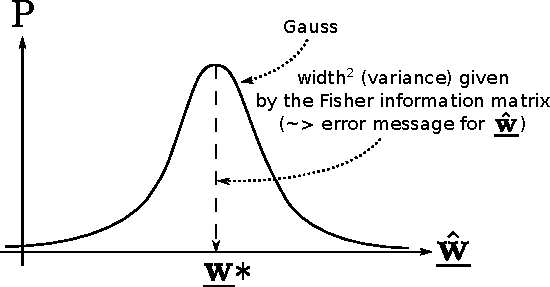
\includegraphics[height=5cm]{section1_fig5}
\end{center}
\begin{itemize}
        \itR ''maximum likelihood'' estimator is asymptotically efficient
                (unbiased \& approaches the Cramer-Rao bound)
        \itR finite number of observations: \\
                maximum likelihood estimator is efficient - if an efficient
                estimator exists\\
                {\it proof: see supplementary material}
        \itR maximum likelihood procedure can often be implemented
        \begin{itemize}
                \itl very practical estimator
        \end{itemize}
\end{itemize}

\paragraph{Summary}\mbox{}\\
\begin{itemize}
   \item An estimator is a random variable.
   \item It can only be analyzed statistically
    (e.g. mean, variance, shape of distribution).
\item biased \& unbiased estimators
\item minimum variance unbiased estimator (MVU) has smallest variance
  for \textbf{all values} of the true parameter
\end{itemize}  

MVUs and the Cramer-Rao bound
\begin{itemize}
\item minimum variance unbiased estimators do not always exist
\item Cramer Rao Bound  provides a universal bound but may not be realizable
\end{itemize}
 
\paragraph{Outlook}\mbox{}\\
  \textbf{Inclusion of prior knowledge}
    
  \begin{itemize}
  \item MLEs: no prior knowledge regarding 'reasonable' parameter values %\pause
  \item Maximum a Posteriori estimates (MAP) incorporate such
    knowledge via Bayes Theorem ($\leadsto$ regularisation)  
  $$p(\vec{w}|\vec{x}) \propto p(\vec{x}|\vec{w}) p(\vec{w})$$
  \item Beyond point estimates: Bayesian statistics. A complete (probabilistic) treatment should exploit the degrees of belief in a given model (set of parameters)
  \end{itemize}


